\chapter{Konzeption}\label{chapter:concept}
Der Inhalt dieses Kapitels stellt die Konzeption eines Testerstellungssystems namens \textit{Unitcraft} zur Bearbeitung des Hauptthemas dar. Dies geschieht in einer nachvollziehbaren Weise, sodass das erstellte Konzept reproduzierbar ist.

\section{Voraussetzungen}
Im Mittelpunkt der Arbeit befindet sich die Programmiersprache Java. Zur Vereinfachung der Analyse und Ausführung der generierten Tests werden die Java-Projekte auf das \textit{Build-Automation-Tool} Apache Maven beschränkt. Hierbei wird die klassische Maven Projektstruktur eingehalten. Diese besteht zunächst aus dem \textit{src}-Verzeichnis, welches sich in das \textit{main}-Verzeichnis, in dem sich der Java-Programmcode bzw. die dazugehörigen Ressourcen befinden, und in das \textit{test}-Verzeichnis unterteilt. \cite{MavenIntroductionStandard} [Abb. \ref{fig:dir}]\\ Somit wird eine klare Trennung zwischen Programmcode und Testcode gewährleistet und deutlich, in welchem Verzeichnis die Tests abgelegt werden müssen. \begin{figure}[h]
    \centering
    \begin{minipage}{4cm}
    \dirtree{%
    .1 src.
    .2 main.
    .3 java.
    .3 resources.
    .2 test.
    .3 java.
    .3 resources.
    }
    \end{minipage}
    \caption{\textit{Maven} Projektstruktur}
    \label{fig:dir}
\end{figure} \newpage
Um ein umfangreiches Generieren von Tests zu ermöglichen, ist die Einbindung von Frameworks als \textit{Dependencies} in der pom.xml essenziell. Neben dem Nutzen von JUnit-Jupiter wird ein Einbinden von Mockito vorausgesetzt, sodass die Verwendung von \textit{mocks} ermöglicht wird.\\
Zur Generierung von Metriken wird SonarQube in das Konzept eingebaut. Dabei wird ein weiteres \textit{Plugin} benötigt, um einen \textit{Coverage-Report} erzeugen zu können. Die \textit{Java Code Coverage Library} (kurz JaCoCo) ermöglicht das Erstellen eines \textit{Code-Reports} und stellt SonarQube alle notwendigen Daten bereit.
Die Implementierung von \textit{Plugins} und \textit{Dependencies} erfolgt im Kapitel \ref{chapter:impl}.

\section{Anforderungsanalyse}\label{section:anford}
Um das Testerstellungssystem praktikabel anwendbar zu gestalten, muss zunächst die Zielgruppe der Arbeit betrachtet werden. Es handelt sich dabei um Personen, die fachlich zugeordnet sind, und somit eine Wissensbasis im Bereich der Informatik besitzen. Aufgrund dessen wird auf eine nutzerfreundliche Oberfläche verzichtet und somit der Fokus auf die Programmlogik gelenkt.\\ Ein Testerstellungssystem als Kommandozeilen-Tool bietet hier eine vereinfachte Anwendung innerhalb des Projekts und eröffnet die Möglichkeit einer zukünftigen Einbindung in Automationsprozesse wie bspw. der \textit{Continuos Integration} (engl. kurz CI).\\ Die Wahl der Programmiersprache fällt hierbei auf Python. Python ist eine \textit{high-level}, interpretierte und dynamische Programmiersprache, welche Vorteile wie bspw. zahlreiche \textit{Libraries} für LLM-Schnittstellen, eine große aktive Community sowie eine einfache Lesbarkeit mit sich bringt. \cite*{PythonLanguageAdvantages2017} Die Umsetzung eines Python-Kommandozeilen-Tools erfordert eine detaillierte Anforderungsanalyse, um die Zielfunktionalitäten zu gewährleisten.\\\\
Um die zu verwendende Prompt-Technik und Temperatur festlegen zu können, wird zu Beginn eine \textbf{Nutzerabfrage zum Initialisieren der Prompt- und Temperaturvariablen} benötigt. Dabei kann zwischen den vorher definierten Promptdesigns gewählt werden. \\ Zur Generierung des Prompts ist es notwendig, das \textbf{Projekt automatisch zu analysieren und alle relevanten Java Klassen zu erfassen}. Dazu muss das \textit{src}-Verzeichnis genutzt werden, da der relevante Programmcode in diesem abgelegt ist.\\ Sind alle Klassen erfasst, müssen wichtige Details extrahiert werden, sodass dem Sprachmodell ein klar definierter Kontext überliefert wird. Dazu gehören folgende Aspekte:
\begin{itemize}
    \setlength{\parskip}{1pt}
    \item \textit{Package}
    \item \textit{Imports}
    \item Name der Klasse
    \item Name der Methode, zu der Tests generiert werden sollen
    \item Konstruktor
    \item Methodeninhalt (Programmcode der Methode)
\end{itemize}
Somit ist es möglich, dem Sprachmodell iterativ alle Methoden in Form eines separaten Prompts mit oben genannten Informationen zu übergeben, um den Fokus und somit den Kontext auf eine einzelne Methode zu setzen. \\ Stehen alle Informationen bereit und wurden korrekt aus der Java-Klasse extrahiert, muss ein \textbf{Prompt erstellt} werden. Der über die Nutzerabfrage gewählte Prompt wird mit den extrahierten Informationen gefüllt und zum Generieren des Testcodes verwendet.\\ Infolgedessen wird eine \textit{Application Programming Interface} (engl. kurz API) Anfrage an die vom Anbieter bereitgestellte \acs{API}, zur Kommunikation mit dem LLM, benötigt. Somit lässt sich das \textbf{Generieren von Testcode über eine API-Anfrage} realisieren.\\ Das Ergebnis der Anfrage bzw. die Antwort des Sprachmodells in Form einer Testklasse auf den gestellten Prompt sollte überprüft werden, bevor diese ins Projekt integriert wird. Eine \textbf{Überprüfung der Kompilierbarkeit der Testklasse} sorgt dafür, dass die Tests überhaupt ausführbar sind und bei späterer Durchführung der Prozess aufgrund eines \textit{Build-} oder Kompilierfehlers nicht scheitert.\\ Treten die eben genannten Fehler auf, sollte dem LLM eine Möglichkeit zur Fehlerbehebung geboten werden. \textbf{Repair Rounds} stellen diesen Aspekt bereit und ermöglichen eine Verbesserung des Testcodes durch die Fehlerbehebung oder Aufforderung, fehlerverursachenden Code oder die komplette Testklasse zu löschen, falls eine Behebung nicht erfolgreich ist. \\ Ist die Kompilierung aller Tests problemlos erfolgt, muss die \textbf{Testklasse in eine Java-Datei geschrieben} und im \textit{test}-\textbf{Verzeichnis abgelegt werden}. Dabei soll der komplette Pfad aus dem \textit{src}-Verzeichnis ins \textit{test}-Verzeichnis übernommen werden, um eine übersichtliche Projektstruktur zu gewährleisten.\\\\Zusammengefasst benötigt \textit{Unitcraft} folgende Zielfunktionalitäten:
\begin{itemize}
    \setlength{\parskip}{1pt}
    \item Nutzerabfrage zum Initialisieren der Prompt- und Temperaturvariablen
    \item Automatisches Erfassen aller Java Klassen
    \item Erstellen eines Prompts
    \item Generieren von Testcode über eine API-Anfrage zur Kommunikation mit dem LLM
    \item Überprüfung der Kompilierbarkeit der Testklasse
    \item \textit{Repair Rounds} zur Fehlerbehebung oder zum Löschen relevanter Codeausschnitte/der Testklasse
    \item Schreiben der Testklasse in Java-Datei und Ablegen im \textit{test}-Verzeichnis mit korrektem Pfad
\end{itemize}
Durch die eben genannten Anforderungen wird eine Evaluation von LLM's hinsichtlich ihrer Eignung zur Generierung von JUnit Tests ermöglicht. Durch Funktionalitäten wie \textit{Repair Rounds} und die Überprüfung der Kompilierbarkeit nähert man sich der Rolle eines manuellen Testers, ohne auf den vom Sprachmodell generierten Code Einfluss zu nehmen. Damit wird eine qualitative Analyse gewährleistet.

\section{Wahl des Large Language Models}
Bereits in Kapitel \ref{subsection:gpt} wurde erklärt, dass die Serie der GPT, speziell die Sprachmodelle von OpenAI, aufgrund ihrer hohen Performance hervorstechen. Vergleicht man die aktuellsten Modelle miteinander, wird deutlich, dass GPT-4o vor allem im \textit{Massive Multi-task Language Understanding} (kurz MMLU) am besten abschneidet. \acs{MMLU} ist ein \textit{Benchmark} für NLP-Modelle, mithilfe dessen sich Fähigkeiten zum Lösen verschiedener Aufgabenstellungen beurteilen lassen. Mit einem Wert von 88.7\% erreicht das GPT-4o Modell die beste Beurteilung. [Abb. \ref{fig:gpt-comp}] \cite{HelloGPT4o} Ebenso Aspekte wie die Aktualität, die verbesserte Geschwindigkeit und der halb so hohe Preis im Vergleich zum aktuellen GPT-4 Modell sprechen für die Verwendung von GPT-4o. \cite{HelloGPT4o} \pgfplotstableread[row sep=\\,col sep=&]{
    GPT & MMLU \\
    GPT-4o & 88.7 \\
    GPT-4T & 86.5 \\
    GPT-4 & 86.4 \\
    }\mydata

\begin{figure}[ht]
    \vspace{0.3cm}
    \centering
    \begin{tikzpicture}
        \begin{axis}[
            ybar,
            width=8.5cm,  % Adjust the width
            height=6cm,  % Adjust the height
            symbolic x coords={GPT-4o, GPT-4T, GPT-4},
            xtick=data,
            ymin=85,  % Set y axis minimum value
            ymax=90,  % Set y axis maximum value
            bar width=20pt,  % Adjust bar width
            nodes near coords,  % Display values on top of bars
            ylabel={MMLU (\%)},
            enlarge x limits=0.5,  % Reduce the space around the bars
        ]
        \addplot table[x=GPT,y=MMLU]{\mydata};
        \end{axis}
    \end{tikzpicture}
    \caption{MMLU-Vergleich der GPT-Modelle}
    \label{fig:gpt-comp}
\end{figure}

\section{Design des Prompts}
Bevor ein Prompt designt werden kann, muss die Prompt-Technik festgelegt werden. Hierbei wird das \textit{Zero-Shot} Prompting sowie \textit{Few-Shot} Prompting in Betracht gezogen. Speziell beim \textit{Few-Shot} Prompting liegt der Fokus auf dem \textit{One-Shot} Prompt, da dieser bei der Generierung von Code Vorteile wie bspw. einem zusätzlichen Beispielkontext mitbringt. Außerdem muss beachtet werden, dass ein Sprachmodell ein begrenztes Kontextfenster in Form von Token besitzt. Somit wäre ein Hinzufügen weiterer Beispielkontexte aufgrund des höheren Tokenverbrauchs für Beispiele ineffektiv und würde die Anzahl an relevanten Codezeilen im Prompt einschränken.\\
Der Aufbau der zu nutzenden Prompts besteht aus verschiedenen Parametern. Das \textit{model} legt fest, an welches Sprachmodell der Prompt gestellt werden soll. Der zweite Parameter ist eine Liste von \textit{messages}, welche an das Modell gesendet werden. Dazu vergibt man pro Nachricht eine \textit{role} sowie einen \textit{content}. Darüber lässt sich die Anweisung an das LLM sowie die verlangte Ausgabe über die \textit{role} ``System'' und die Eingabedaten bzw. ein zusätzlicher Kontext des Users über die \textit{role} ``User'' realisieren. Der Temperaturparameter legt die Kreativität fest und \textit{max tokens} die maximale Anzahl an Tokens, die dem Sprachmodell für den Output zur Verfügung gestellt werden.\\
Insbesondere die Parameter \textit{model}, \textit{temperature} und \textit{max tokens} unterscheiden sich zwischen beiden Prompt-Techniken nicht. Da wir das Sprachmodell GPT-4o nutzen, wird das \textit{model} mit dem String ``gpt-4o'' initialisiert. Die Temperatur wird über eine Nutzerabfrage festgelegt, welche den Wert 0, 0.25 und 0.5 vorgibt, da vor allem präzise Aufgaben wie die Codegenerierung eine niedrige Temperatur erfordern, um gute Ergebnisse zu erzielen. \cite*{renzeEffectSamplingTemperature2024} Somit wird durch 0 ein deterministischer Wert und 0.5 ein Wert mit Kreativitätsanteil bereitgestellt. Um die Ausgabe nicht einzuschränken setzen wir \textit{max tokens} auf den maximalen Output Wert. Im Falle von GPT-4o ist dieser 4096 Token. Beide Prompt-Techniken erhalten ebenso die in Abbildung \ref{fig:system} dargestellte Systemanweisung.\begin{figure}[ht]
    \vspace{.5cm}
    \centering
    \tikzstyle{block} = [rectangle, draw, text width=25em, inner sep=1ex, rounded corners, font=\small]
    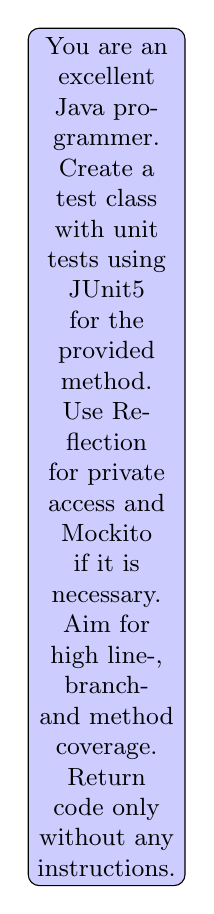
\begin{tikzpicture}
        \tikzset{node distance = 0.75cm and 1.5cm}
        % Main node with embedded tikzpicture
        \node (n1) at (0,0) [block] {
            You are an excellent Java programmer. Create a test class with unit tests using JUnit5 for the provided method. Use Reflection for private access and Mockito if it is necessary. Aim for high line-, branch- and method coverage. Return code only without any instructions.
};
    \end{tikzpicture}
    \caption{Sytemanweisung}
    \label{fig:system}
\end{figure}
Die Anweisung deckt alle wichtigen Aspekte wie bspw. die Hauptaufgabe, das Ziel, die zu verwendenden Technologien sowie das Ausgabeformat ab. \\
Der \textit{Zero-Shot} Prompt und der \textit{One-Shot} Prompt unterscheiden sich in den bereitgestellten Daten. Die Eingabedaten für den \textit{Zero-Shot} Prompt sieht man in Abbildung \ref{fig:content-0}.\begin{figure}[H]
    \vspace{.5cm}
    \centering
    \tikzstyle{block} = [rectangle, draw, text width=25em, inner sep=1ex, rounded corners, font=\small]
    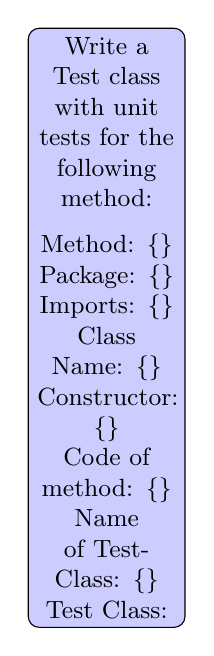
\begin{tikzpicture}
        \tikzset{node distance = 0.75cm and 1.5cm}
        % Main node with embedded tikzpicture
        \node (n1) at (0,0) [block] {
            Write a Test class with unit tests for the following method: \\[0.2cm]
            Method: \{\}\\
            Package: \{\}\\
            Imports: \{\}\\
            Class Name: \{\}\\
            Constructor: \{\}\\
            Code of method: \{\}\\
            Name of TestClass: \{\}\\
            Test Class:
};
    \end{tikzpicture}
    \caption{\textit{Zero-Shot} Prompt Eingabedaten}
    \label{fig:content-0}
\end{figure}
Hierbei werden neben einer zusätzlichen Anweisung alle in Kapitel \ref{section:anford} aufgezeigten Informationen der Java-Klasse bereitgestellt. Die geschweiften Klammern werden durch die extrahierten Daten ersetzt. Auch im \textit{One-Shot} Prompt werden die Eingabedaten unter Abbildung \ref{fig:content-0} verwendet. Hinzu kommt jedoch der zusätzliche Beispielkontext wie in Abbildung \ref{fig:content-1} zu erkennen.\begin{figure}[H]
    \centering
    \tikzstyle{block} = [rectangle, draw, text width=25em, inner sep=1ex, rounded corners, font=\small]
    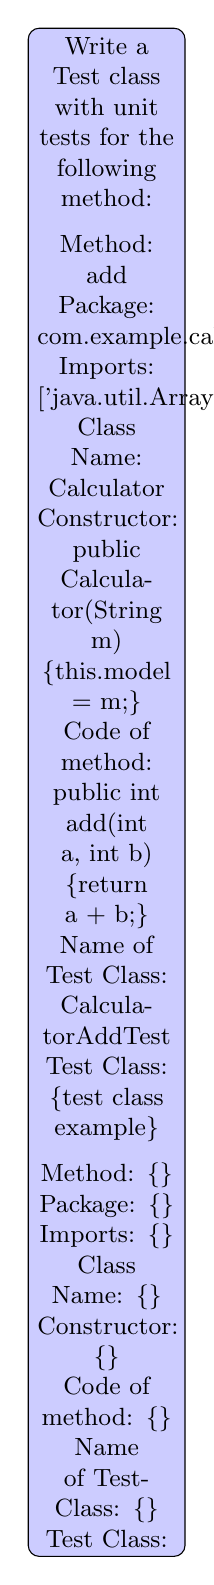
\begin{tikzpicture}
        \tikzset{node distance = 0.75cm and 1.5cm}
        % Main node with embedded tikzpicture
        \node (n1) at (0,0) [block] {
            Write a Test class with unit tests for the following method: \\[0.2cm]
            Method: add\\
            Package: com.example.calculator\\
            Imports: ['java.util.ArrayList']\\
            Class Name: Calculator\\
            Constructor: public Calculator(String m) \{this.model = m;\}\\
            Code of method: public int add(int a, int b) \{return a + b;\}\\
            Name of Test Class: CalculatorAddTest\\
            Test Class: \{test class example\}\\[0.2cm]        
            Method: \{\}\\
            Package: \{\}\\
            Imports: \{\}\\
            Class Name: \{\}\\
            Constructor: \{\}\\
            Code of method: \{\}\\
            Name of TestClass: \{\}\\
            Test Class:
};
    \end{tikzpicture}
    \caption{\textit{One-Shot} Prompt Eingabedaten (mit Zusatzkontext)}
    \label{fig:content-1}
    \vspace{-.5cm}
\end{figure}
Die entsprechende Testklasse zum Beispielkontext stellt Quellcode \ref{lst:test-class-context} dar.\\
\lstinputlisting[caption=Testklasse für Beispielkontext,captionpos=b,label={lst:test-class-context},language=Java]{Assets/Code/TestClass.java}\vspace{-.3cm} Dadurch wird beispielhaft gezeigt, wie die bereitgestellten Informationen verarbeitet und verwendet werden können, um eine Testklasse zu erzeugen. Bei beiden Prompt-Techniken wird die Test Klasse der Eingabedaten leer gelassen, sodass dem LLM noch einmal das Generieren einer solchen Klasse signalisiert wird.\\
Zur Nutzung von \textit{Repair Rounds} werden jedoch weitere Anweisungen benötigt. Dazu gehört das Beheben von Kompilierfehlern [Abb. \ref{fig:system-repair}] und das Löschen von fehlerhaften Codezeilen [Abb. \ref{fig:system-delete}].\begin{figure}[ht]
    \vspace{.5cm}
    \centering
    \tikzstyle{block} = [rectangle, draw, text width=25em, inner sep=1ex, rounded corners, font=\small]
    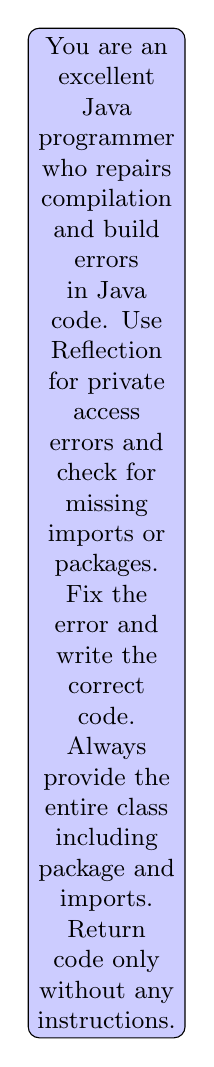
\begin{tikzpicture}
        \tikzset{node distance = 0.75cm and 1.5cm}
        % Main node with embedded tikzpicture
        \node (n1) at (0,0) [block] {
            You are an excellent Java programmer who repairs compilation and build errors in Java code. Use Reflection for private access errors and check for missing imports or packages. Fix the error and write the correct code. Always provide the entire class including package and imports. Return code only without any instructions.
};
    \end{tikzpicture}
    \caption{Sytemanweisung zum Beheben von Kompilierfehlern}
    \label{fig:system-repair}
\end{figure}
\begin{figure}[ht]
    \vspace{.5cm}
    \centering
    \tikzstyle{block} = [rectangle, draw, text width=25em, inner sep=1ex, rounded corners, font=\small]
    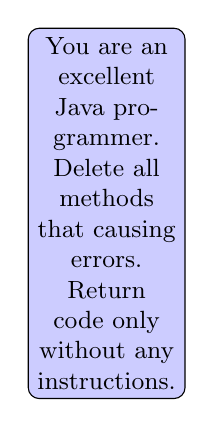
\begin{tikzpicture}
        \tikzset{node distance = 0.75cm and 1.5cm}
        % Main node with embedded tikzpicture
        \node (n1) at (0,0) [block] {
            You are an excellent Java programmer. Delete all methods that causing errors. Return code only without any instructions.
};
    \end{tikzpicture}
    \caption{Sytemanweisung zum Löschen fehlerhafter Codezeilen}
    \label{fig:system-delete}
\end{figure}
Beide Anweisungen nennen die Hauptaufgabe und legen den Fokus auf die spezifizierte Anforderung. Es werden ebenso Technologieempfehlungen angesprochen und der Ausgabeindikator festgesetzt. Als Eingabedaten dienen lediglich der generierte Testcode mit dazugehöriger Error-Meldung, was dem \textit{Zero-Shot} Prompting entspricht. Auch die Parameter für \textit{model}, \textit{max tokens} und \textit{temperature} entsprechen denen der vorherigen Prompts.\\
Somit wurden 4 verschiedene Prompts designt. Der \textit{Zero-Shot} Prompt sowie \textit{One-Shot} Prompt für das Generieren der Tests und zwei \textit{Zero-Shot} Prompts zum Beheben von Fehlern bzw. Löschen von Codezeilen. 

\section{Programmablaufplan}
Um einen qualitativen Testgenerierungsprozess zu gewährleisten, soll \textit{Unitcraft} nach dem in Abbildung \ref{fig:pap} gezeigten Programmablaufplan erstellt werden. Dieser beschreibt die Folge an Operationen die für die Generierung der Tests und das Erreichen der Zielfunktionalitäten in Kapitel \ref{section:anford} notwendig sind.\tikzset{decision/.style = {diamond, draw, fill=yellow!20, 
		text width=4em, text centered, node distance=3cm, inner sep=0pt},
	block/.style = {rectangle, draw, fill=blue!20, 
		text width=5em, minimum width=3em, text centered, rounded corners, minimum height=3.5em},
	line/.style = {draw, -latex'},
	cloud/.style = {draw, ellipse,fill=red!20, node distance=1cm,
  		minimum height=2em},
	process/.style = {rectangle, draw, fill=green!20, 
		text width=5em, text centered, rounded corners, minimum height=2em},
	input/.style = {trapezium, trapezium left angle=75, trapezium right angle=105, draw, fill=orange!20, 
		text width=5em, text centered, minimum height=2em},
		every node/.append style = {font=\small},}

\begin{figure}[H]
	\vspace{.3cm}
    \centering
    \begin{tikzpicture}[node distance = 1cm, auto]
        % Place nodes
        \node [cloud] (start) {\textbf{Start}};
        \node [input, right of=start, node distance=3cm] (init) {Eingabe von T/Prompt-Technik};
		\node [block, right of=init, node distance=3.5cm] (get) {Erfasse Java-Dateien im Projekt};
		\node [decision, below of=get, node distance=3cm, fill=green!20] (vor) {vorhanden?};
		\node [block, below of=init, node distance=3cm] (extr) {Extrahieren aller Infos};
		\node [cloud, right of=vor, node distance=2.75cm] (stop) {\textbf{Stop}};
		\node [block, left of=extr, node distance=3cm] (api) {API-Anfrage für Testgenerierung};
		\node [decision, below of=api, node distance=2.5cm, fill=green!20] (comp) {kompilierbar?};
		\node [block, below of=comp, node distance=2.5cm] (direct) {Ablegen in Testpfad};
		\node [block, right of=comp, node distance=2.5cm, text width=2.5em] (i) {$i=1$};
		\node [block, right of=i, node distance=2.5cm] (repair) {API-Anfrage zum Reparieren};
		\node [decision, below of=repair, node distance=2.5cm, fill=green!20] (comp1) {kompilierbar?};
		\node [block, right of=comp1, node distance=2.75cm, text width=3.5em] (incr) {$i=i+1$};
		\node [decision, right of=incr, node distance=2.5cm, fill=green!20] (less) {$i\leq2?$};
		\node [block, below of=less, node distance=2.25cm] (apidel) {API-Anfrage zum Löschen};
		\node [decision, below of=apidel, node distance=2.5cm, fill=green!20] (comp2) {kompilierbar?};
		\node [block, left of=comp2, node distance=3.25cm] (del) {Löschen};
		\node [decision, below of=direct, node distance=2.5cm, fill=green!20] (file) {\footnotesize{weitere Datei?}\vspace{.1cm}};
		\node [cloud, below of=file, node distance=2.25cm] (end) {\textbf{Stop}};

		\path [line] (start) -- (init);
		\path [line] (init) -- (get);
		\path [line] (vor) -- node [pos=0.4] {N} (stop);
		\path [line] (get) -- (vor);
		\path [line] (vor) -- node [pos=0.4] {J} (extr);
		\path [line] (extr) -- (api);
		\path [line] (api) -- (comp);
		\path [line] (comp) -- node [pos=0.4] {J} (direct);
		\path [line] (comp) -- node [pos=0.4] {N} (i);
		\path [line] (i) -- (repair);
		\path [line] (repair) -- (comp1);
		\path [line] (comp1) -- node [pos=0.4] {J} (direct);
		\path [line] (comp1) -- node [pos=0.4] {N} (incr);
		\path [line] (incr) -- (less);
		\path [line] (less) -- node [pos=0.4] {J} ($(less.north) + (0.0cm, 1.25cm)$) |- ($(repair.east)$);
		\path [line] (less) -- node [pos=0.4] {N} (apidel);
		\path [line] (apidel) -- (comp2);
		\path [line] ($(comp2.south)$) -- ($(comp2.south) + (0.0cm, -0.05cm)$) |- node {J} ($(comp2.south) + (-12.0875cm, -0.05cm)$) |- (direct);
		\path [line] (comp2) -- node [pos=0.4] {N} (del);
		\path [line] (direct) -- (file);
		\path [line] (file) -- node [pos=0.4] {N} (end);
		\path [line] ($(del.north)$) -- ($(del.north) + (0.0cm, 1.25cm)$) |- ($(file.east)$);
		\path [line] ($(file.west)$) -- node [pos=0.4] {J} ($(file.west) + (-0.58cm, 0.0cm)$) |- ($(api.west) + (-0.58cm, 1.245cm)$) |- ($(extr.north) + (0.0cm,0.5cm)$) -| (extr);
    \end{tikzpicture}
    \caption{Programmablaufplan von \textit{Unitcraft}}
	\label{fig:pap}
\end{figure}Zunächst findet über die Nutzerabfrage eine Initialisierung der Temperatur und Prompt-Technik statt. Im Anschluss wird das Projekt analysiert und alle Java-Dateien aus dem \textit{src}-Verzeichnis erfasst. Ist dieses Verzeichnis leer oder es existieren keine Java-Dateien, endet das Programm. Im anderen Falle werden die Informationen aller Java-Dateien iterativ extrahiert sowie die entsprechenden Testklassen generiert.\\Der Prozess der Testgenerierung startet mit einer API-Anfrage an die OpenAI-API, in dem mithilfe erfasster Parameter ein Prompt gestellt wird. Sollte die Antwort vom Sprachmodell kompilierbar sein, so wird die Testklasse als Java-Datei im Testpfad abgelegt und das Programm fährt mit der nächsten Java-Datei fort, insofern diese existiert. Andernfalls endet das Programm an dieser Stelle.\\Tritt ein Kompilierfehler o.Ä. auf, startet der Prozess der \textit{Repair Rounds}. Dieser beginnt ebenso mit einer API-Anfrage an die OpenAI-API, in welcher der Prompt zur Reparatur genutzt wird. Sollte die Antwort kompilierbar sein, so wird die Testklasse als Java-Datei im Testpfad abgelegt. Tritt erneut ein Kompilierfehler auf erfolgt eine neue \textit{Repair Round}. Insgesamt gibt es die Möglichkeit auf 2 Runden.\\Ist diese erschöpft, erfolgt eine letzte API-Anfrage an die OpenAI-API zum Löschen der fehlerhaften Codezeilen, sodass der funktionierende Restcode nicht verloren geht.\\Tritt auch danach wieder ein Kompilierfehler auf, wird die komplette Testklasse von \textit{Unitcraft} gelöscht und der Prozess fährt bei der nächsten Java-Datei fort bzw. das Programm endet, falls keine Java-Datei mehr vorhanden ist.